\documentclass[12pt]{article}
\usepackage{float}
\usepackage{xcolor}
\usepackage{newpxtext,euler}
\usepackage[OT1]{fontenc}
\usepackage[spanish]{babel}
\usepackage{amsfonts,amsmath,amssymb,amsthm}
\usepackage{geometry}
\usepackage{bm} % for \bm
\usepackage{fixmath}

\newcommand\N{\ensuremath{\mathbb{N}}}
\newcommand\R{\ensuremath{\mathbb{R}}}
\newcommand\Z{\ensuremath{\mathbb{Z}}}
\renewcommand\O{\ensuremath{\emptyset}}
\newcommand\Q{\ensuremath{\mathbb{Q}}}
\newcommand\C{\ensuremath{\mathbb{C}}}
\newcommand\T{\mathbb{T}}
\renewcommand{\epsilon}{\varepsilon}
\renewcommand{\hat}{\widehat}
\newcommand\jk{\langle k\rangle}


\setlength{\parindent}{0pt}


%!TEX root = main.tex
% Tcolorboxes
\makeatother
\usepackage{thmtools}
\usepackage[framemethod=TikZ]{mdframed}
\mdfsetup{skipabove=1em,skipbelow=1em,nobreak=true}

\theoremstyle{definition}
\declaretheoremstyle[
    headfont=\bfseries\sffamily\color{black!70!black}, bodyfont=\normalfont,
    mdframed={
        linewidth=1pt,
        rightline=true, topline=true, bottomline=true,
        linecolor=black, backgroundcolor=black!0!white,
    }
]{thmbox}
\declaretheoremstyle[
    headfont=\bfseries\sffamily\color{black!70!black}, bodyfont=\normalfont,
    mdframed={
        linewidth=1pt,
        leftline=false,rightline=false, topline=false, bottomline=false,
        linecolor=black, backgroundcolor=black!0!white,
    }
]{standar}


\declaretheoremstyle[
    headfont=\bfseries\sffamily\color{black!70!black}, bodyfont=\normalfont,
    numbered=no,
    qed=\qedsymbol
]{thmproofbox}

\declaretheorem[numberwithin=section,style=thmbox, name=Definición]{definition}
\declaretheorem[sibling=definition,style=standar, numbered=no, name=Ejemplo]{eg}
\declaretheorem[sibling=definition,style=thmbox, name=Proposición]{prop}
\declaretheorem[sibling=definition,style=thmbox, name=Teorema, numbered=yes]{theorem}
\declaretheorem[sibling=definition,style=thmbox, name=Lema]{lemma}
\declaretheorem[sibling=definition,style=thmbox, name=Corolario]{corollary}

\declaretheorem[style=thmproofbox, name=Demostración]{replacementproof}
\renewenvironment{proof}[1][\proofname]{\vspace{-10pt}\begin{replacementproof}}{\end{replacementproof}}

\declaretheorem[style=standar, numbered=no, name=Nota]{note}


\newcommand{\bb}[1]{\mathbb{#1}}

\usepackage[most]{tcolorbox}
\tcbuselibrary{most}

\tcbset {
  base/.style={
    arc=7mm, 
    bottomtitle=0.5mm,
    boxrule=0mm,
    colbacktitle=black!90!white, 
    coltitle=white, 
    fonttitle=\bfseries, 
    left=2.5mm,
    leftrule=1mm,
    right=3.5mm,
    title={#1},
    toptitle=0.75mm, 
  }
}


\newtcolorbox{subbox}[1]{
  colframe=black!93!white,
  base={#1}
}
\usepackage{lipsum}
 \geometry{
 a4paper,
 total={170mm,260mm},
 left=20mm,
 top=15mm,
 }
 
\title{\vspace{-2cm}\par\noindent\rule{16cm}{1pt}\large
\\\bfseries BioCódigos
\vspace{-0.34cm}\par\noindent\hspace{0.15cm}\rule{16cm}{1pt}
\vspace{-0.6cm}
}
\author{\small \bfseries María Alejandra Rodríguez Ríos$.^1$\quad \quad\small Edgar Santiago Ochoa Quiroga$.^{2}$\\ \small \quad \texttt{mrodriguezri@unal.edu.co} \quad \quad \quad \quad \quad \quad \texttt{eochoaq@unal.edu.co}\quad\quad \quad\\ \small \bfseries Saul Alvarez Lazaro$^{3}$\\
\small \texttt{salvarezla@unal.edu.co}
}

\usepackage{titling}
\predate{\hspace{6.24cm}\small}
\postdate{}

\begin{document}


\maketitle
\begin{abstract}
Este proyecto tiene como objetivo hacer un primer acercamiento a la Teoría de Códigos del ADN, en particular se abordaran los códigos de Hamming y Reed-Solomon y como estos se relacionan con la codificación genética, ademas se harán implementaciones de algunos casos particulares que fueron hallados en la investigación. Por ultimo se hará un análisis de el desempeño de las simulaciones y posibles maneras de continuar por esta linea de investigación.
\end{abstract}

\section{Introducción}

%!TEX root = main.tex

La Teoría de la Codificación y la Teoría de la Información, vistas desde las matemáticas, surgieron a partir de ideas relativamente recientes y, dentro del esquema matemático, se consideran disciplinas modernas. Desde esta perspectiva, la implementación de cadenas biológicas para el almacenamiento de información es aún más innovadora, dado que sus primeros desarrollos se remontan a finales del siglo XX e inicios del siglo XXI.\\

Uno de los principales objetivos de este campo emergente es estudiar los procesos biológicos y explorar posibles formas de almacenamiento de datos en ellos. Este enfoque es altamente ambicioso y requiere herramientas avanzadas. Por ello, el propósito de este trabajo es realizar un primer acercamiento al estudio de estos procesos, analizando su comportamiento, estableciendo paralelismos entre los mecanismos biológicos y los códigos correctores de errores, y presentando algunas implementaciones para su simulación y visualización.



\section{Preliminares}
En esta sección, se abordarán los conceptos preliminares relacionados con el ADN y su proceso biológico de transcripción y traducción, así como una introducción a los códigos de corrección de errores, específicamente los códigos de Hamming y los códigos de Reed-Solomon.
\subsection{ADN y el proceso de replicación, transcripción y traducción}
%!TEX root = main.tex

El ácido desoxirribonucleico (ADN) es una molécula fundamental presente en el interior de las células tanto eucariotas como procariotas, que contiene la información genética necesaria para el desarrollo, funcionamiento y reproducción de los organismos. Esta molécula permite la transmisión de la información genética de una generación a la siguiente. Su estructura es una doble hélice, formada por enlaces débiles de hidrógeno que unen las bases nitrogenadas de los nucleótidos purínicos y pirimidínicos, los cuales se enrollan alrededor de un eje central. Cada nucleótido está compuesto por un esqueleto de azúcar desoxirribosa y grupos fosfato, conectados mediante las bases nitrogenadas.\\

En cuanto a la historia del descubrimiento de la estructura del ADN, se sabe que fue inicialmente identificada por la científica Rosalind Franklin, quien a través de la técnica de difracción de rayos X obtuvo fotografías que revelaban la forma helicoidal de la molécula. Sin embargo, su contribución no fue reconocida en su momento. Fue solo cuando James Watson y Francis Crick, científicos que trabajaban en el Laboratorio Cavendish, utilizaron esas imágenes y algunas de las deducciones previas para publicar, en 1953, el artículo que describía la estructura del ADN. Años después, Watson y Crick recibieron el Premio Nobel de Medicina por este descubrimiento, pero nunca se le otorgó el reconocimiento que le correspondía a Rosalind Franklin.\\

Respecto a la estructura molecular, se sabe que el ADN está formado por cuatro elementos fundamentales: los nucleótidos adenina (A), guanina (G), timina (T) y citosina (C). Los dos primeros corresponden a los nucleótidos purínicos y los dos restantes son pirimidínicos. Estas bases nitrogenadas se emparejan de manera específica: la adenina se empareja con la timina y la guanina con la citosina. Este emparejamiento es esencial para la estabilidad y la función del ADN, permitiendo una transmisión precisa de la información genética.La importancia del ADN radica en que es esencial para los procesos que la célula utiliza para elaborar todas las proteínas que un ser vivo necesita para subsistir. Estos procesos de transmisión de información se realizan en tres etapas, a las cuales se denomina el dogma central de la biología molecular. Este concepto describe el flujo de información genética en una célula, estableciendo que la información genética fluye desde el ADN, a través de la síntesis de ARN, y luego a través de la síntesis de proteínas.\\

Para poder realizar el paso de ADN a ARNm o ácido ribonucleico mensajero, necesitamos pasar por el proceso de replicación. La replicación es el proceso mediante el cual una célula copia su ADN para asegurar que cada célula hija reciba una copia exacta de la información genética. Este proceso es esencial para la división celular y tiene lugar antes de que una célula se divida, durante la fase S del ciclo celular. Uno de los primeros pasos en la replicación es cuando se desenrolla la doble hélice del ADN, lo cual es realizado por una clase de enzimas conocidas como helicasas. Las helicasas tienen la función de romper los enlaces de hidrógeno que mantienen unidas las bases nitrogenadas de las dos cadenas complementarias de ADN, separándolas y formando lo que se conoce como la horquilla de replicación.\\

Es importante entender que el ADN es una molécula en la que sus dos cadenas tienen orientaciones opuestas. Una cadena se lee en la dirección 5' a 3', mientras que la otra se lee en la dirección opuesta, es decir, 3' a 5'. Esto se refiere a los extremos de las cadenas de ADN: el extremo 5' de una cadena de ADN tiene un grupo fosfato unido al quinto carbono del azúcar, mientras que el extremo 3' tiene un grupo hidroxilo unido al tercer carbono del azúcar.Una vez que se forma la horquilla de replicación, las dos cadenas de ADN están abiertas y disponibles para ser copiadas. Sin embargo, la lectura y la síntesis del ADN no son simétricas, ya que la ADN polimerasa, la enzima encargada de sintetizar nuevas cadenas de ADN, solo puede agregar nucleótidos en la dirección 5' a 3'.\\

Ahi inicia el segundo paso el cual es la transcripción, en este la información genética contenida en el ADN se transcribe a una molécula de ARN mensajero (ARNm). Este proceso ocurre en el núcleo de las células eucariotas y en el citoplasma de las procariotas y es esencial para la posterior síntesis de proteínas. La transcripción comienza cuando la enzima ARN polimerasa se une a una región específica del ADN conocida como el promotor. El promotor es una secuencia de bases que indica el inicio de un gen y es crucial para la correcta transcripción del ADN. Una vez que la ARN polimerasa se une al promotor, comienza a desenrollar la doble hélice del ADN y a leer la cadena de ADN en la dirección 3' a 5'.\\

A medida que la ARN polimerasa avanza, sintetiza una cadena de ARN mensajero (ARNm) complementaria a la cadena molde del ADN. Durante este proceso, las bases del ADN se emparejan de forma específica con los ribonucleótidos, la adenina (A) del ADN se empareja con el uracilo (U) en el ARN , la citosina (C) con la guanina (G). El resultado es una nueva cadena de ARN que lleva la misma información genética que el ADN, pero en una forma que puede ser utilizada en la síntesis de proteínas.\\

La ARN polimerasa sigue leyendo el ADN hasta llegar a una secuencia de terminación que indica el final del gen. En este punto, la transcripción finaliza, y el ARN mensajero (ARNm) recién formado se separa del ADN. El ARNm, que ahora contiene la "copia" de la información genética, es transportado fuera del núcleo hacia los ribosomas en el citoplasma, donde se llevará a cabo la siguiente etapa.\\

Por último tenemos la traducción, este es el proceso  comienza cuando el ARNm se une a un ribosoma en el citoplasma. El ribosoma lee el ARNm en bloques de tres bases nitrogenadas consecutivas, llamados códones. Cada códon especifica un aminoácido particular, que es la unidad básica de las proteínas. Existen 64 posibles combinaciones de códones, que codifican para 20 aminoácidos diferentes, lo que permite una gran diversidad en la construcción de proteínas.\\

El ARN de transferencia ARNt  tiene un anticódon, el cual es una secuencia de tres bases que es complementaria a un códon del ARNm en uno de sus extremos y un aminoácido específico en el otro extremo. A medida que el ribosoma lee el ARNm, el ARNt transporta el aminoácido correspondiente al códon leído y lo coloca en la cadena polipeptídica en crecimiento. Este proceso se repite a medida que el ribosoma avanza a lo largo del ARNm. La traducción continúa hasta que el ribosoma encuentra un códon de terminación en el ARNm, lo que indica el final de la síntesis de la proteína. En ese momento, la cadena polipeptídica recién formada se libera, y la proteína se pliega para adoptar una estructura funcional.\\

Sin embargo, este proceso no siempre se lleva a cabo sin errores, por lo cual se tienen mecanismos que buscan corregir la mayoría de los errores que pueden surgir puesto que el no corregirlos por ejemplo en los humanos puede verse reflejado en mutaciones genéticas, proteínas no funcionales o mal plegadas y a la pérdida de la integridad genética, lo que puede causar disfunción en todo el organismo.\\

\subsubsection{Corrección de errores}


Los procesos de replicación, transcripción y traducción son fundamentales para la correcta expresión de la información genética. Sin embargo, a lo largo de estos procesos pueden ocurrir errores, como la inserción de bases incorrectas o la incorrecta traducción de los codones. Para eso existen mecanismos de corrección para asegurar la fidelidad genética y evitar que estos errores afecten a la célula.\\

La replicación del ADN es un proceso crítico para la división celular. Sin embargo, es común que durante la síntesis de las nuevas cadenas de ADN se produzcan errores en la incorporación de nucleótidos. Para corregir estos errores, la ADN polimerasa tiene una función de corrección por prueba de lectura. Esta actividad se realiza mediante la exonucleasa 3' a 5', una función de la propia enzima que le permite retroceder y eliminar los nucleótidos incorrectos que acaba de incorporar, reemplazándolos por los correctos.\\

De igual manera, en la transcripción para la corrección de errores el ARN polimerasa también posee mecanismos de corrección para detectar y corregir ciertos errores en el ARNm durante su síntesis, como lo es retirar el nucleótido equivocado y poner el correcto en su lugar\\

En la traducción también pueden ocurrir errores, como la incorporación de un aminoácido incorrecto debido a un códon mal leído o a un error en el emparejamiento entre el ARNm y el ARNt. Para esto, los ribosomas tienen mecanismos de verificación para asegurar que la secuencia de aminoácidos sea correcta, por ejemplo, el anticódon del ARNt debe coincidir exactamente con el códon del ARNm para que el aminoácido correcto se incorpore en la proteína en formación.\\

Otros errores que se pueden presentar en este proceso que no son por un cambio de nucleótido, sino por un daño en la estructura o un espacio sin nucleótido, para estos existe mecanismos como la reparación por escisión de bases y la reparación por escisión de nucleótidos, este es un mecanismo que se usa para detectar y eliminar ciertos tipos de bases dañadas mediante un grupo de enzimas llamadas glicosilasas, donde cada glicosilasa detecta y elimina un tipo específico de base dañada.\\
\subsection{Códigos de Corrección de Errores.}
De manera similar, cuando enviamos un mensaje a través de un canal, queremos que el receptor de aquel mensaje lo reciba de manera mas fidedigna posible, pero enviar el mensaje puede que la información se vea alterada por el canal, de esta manera la intención detrás de este tipo de códigos como lo indica su nombre es la de ser capaces de detectar los errores en el mensaje recibido, y de corregirlos, de esta manera el mensaje sera enviado con éxito completamente.

En esta sección daremos los hechos mas relevantes de los códigos que utilizaremos para realizar la codificación y decodificación de cadenas de ADN. No mostraremos las pruebas de los resultados teóricos usados, debido a que este no es el propósito, pero estos hechos pueden ser encontrados en (agregar bibliografia)
%!TEX root = main.tex

\subsubsection{Codigos de Reed-Solomon}
Como fue mencionado antes uno de los dos códigos que utilizaremos en este proyecto, son los códigos de Reed-Solomon. Primero debemos definirlos y para esto los introduciremos por medio de la definición dada en (insertar cita sarria)
\begin{definition}
Dado el cuerpo $GF(D)^n$, donde $k\leq n\leq D$ son enteros positivos. Definimos el código de dimensión $k$ como 
$$RS_D(\alpha,n,k)=\{(f(\alpha_1),\ldots ,f(\alpha_n)):f\in GD(D)[x], grad(f)\leq k-1\}.$$ 
Donde $\alpha=(\alpha_1,\ldots,\alpha_n)\in GF(D)^n$, con componentes distintas. La función de codificación esta dada por
$$(a_0,a_1,\ldots,a_{k-1})\mapsto \left(\sum_{i=0}^{k-1}a_i\alpha_1^{i},\ldots,\sum_{i=0}^{k-1}a_i\alpha_n^{i}\right).$$
Donde cada $a_i\in GF(D).$
\end{definition}
La idea detrás de la construcción de este tipo de código es hacer uso de que un polinomio se encuentra determinado por sus coeficientes. Para ver esto en acción, realicemos un ejemplo sencillo para ver esto en acción
\begin{eg}
     Consideremos un código con $k=2,n=3$ y $D=3.$ Tomamos $\alpha=(0,1,2)$, esto debido a que necesitamos que las entradas sean diferentes por definicion, Note que las tuplas las escribiremos como cadenas de simbolos de ahora en adelante, es decir $(0,1,2)=012$. Luego el codigo esta dado por evaluar en todos los polinomios de grado $1$ con coeficientes en $GF(3).$

     $$RS(2,3,012)=\{000,111,222,012,120,210,021,102,210\}.$$

     En particular si por ejemplo queremos codificar la palabra $12$, que arroja una fuente triaria tenemos que
     $$12\mapsto (1+2\cdot0,1+2\cdot1,1+2\cdot2)=102.$$ 
 \end{eg} 

 Con este ejemplo  podemos enfatizar algunos conceptos
     \begin{itemize}
         \item Si uno quiere codificar palabras de longitud $k$, necesitamos que el campo base tenga mas elementos, es decir si queremos codificar una fuente $4-aria$, necesitamos trabajar mínimo con el cuerpo de finito de 4 elementos o mas.
         \item Note que en este caso la elección del $\alpha$ no es única ya que pudimos haber seleccionado $201,$ por lo que si bien el código bloque cumple la misma función, la codificación cambia. Por lo que seria bueno poder codificar independientemente del $\alpha$ escogido.
         \item  El punto anterior tiene sentido al considerar que la codificación esta completamente determinada por el polinomio al que es asignado la palabra que emite la fuente. 
         
     \end{itemize}

En vista de eso, resulta natural preguntarse si podemos definir los códigos de Reed-Solomon sin considerar un $\alpha$ explicito, es decir, concentrarnos unicamente en la estructura polinomial. Para esto debemos hacer uso de algunos conceptos algebraicos.

\begin{definition}
    Dado el cuerpo finito $GF(D)$, decimos que $\alpha\in GF(D)-\{0\},$ es un elemento primitivo, si $\alpha$ es un generador de $\alpha\in GF(D)-\{0\}$ visto como grupo bajo la operación de multiplicación.  
\end{definition}

Este concepto de elemento generador sera crucial, en el sentido de que si bien con la definición original podemos plantear una matriz generadora $G$ y una de corrección $H$, ahora que trabajaremos con el elemento $\alpha$ en ``abstracto''. Generaremos el código por medio de un polinomio generador. Antes de eso mencionaremos los hechos algebraicos que sustentan esta construcción
\begin{prop}
    Dado el cuerpo $GF(p)$ con $p$ un numero primo, podemos construir el cuerpo $GF(p^e)$ por medio de el cociente $GF(p)/\langle x^{p^e}-x\rangle$.
\end{prop}
esto nos da una construcción por medio de clases de equivalencia, que podemos tomar por medio de residuos, pero resultaría engorrosa, por lo que estos para ejemplificar campos, los construiremos por medio de tomar un factor irreducible de ese polinomio sobre el cuerpo base. El siguiente hecho nos da una caracterización, de aquellos elementos primitivos que podemos ver como raíces del polinomio.
\begin{prop}
    Dado $\alpha\in GF(p^e)$, tenemos que $\alpha^{p^e}-\alpha=0$, luego 
    $$x^{p^e}-x=\prod_{\alpha\in GF(p^e) }(x-\alpha).$$
\end{prop}
Note que si excluimos el elemento $0$, tenemos una factorización sobre los elementos no nulos de nuestro cuerpo finito. Con todos estos ingredientes procedemos a dar la definición que usaremos para la codificación
\begin{definition}
  Dado $\alpha$ un elemento primitivo, el código de Reed-Solomon se define como
  $$RS(n,k)=\{(f(1),f(\alpha),\ldots,f(\alpha^{n-1}))\in GF(D)^n:f\in GF(D)[x], grad(f)\leq k-1\}.$$
  Donde escogemos enteros positivos $n=D-1$ y $k<D.$
\end{definition}
Notemos que en primera instancia pareciera que no hay diferencia en los códigos, pero antes de proceder con la diferencia crucial, algunas observaciones.
\begin{itemize}
    \item Note que bajo esta definición, por el uso del elemento primitivo $\alpha$, a diferencia de la primera definición evaluación, ya no tenemos el elemento $0$ considerado.
    \item Ejemplos pequeños como el realizado para la anterior definición, ya no son viables debido a la restricción de la evaluación en elementos primitivos.
    \item Note que antes había mas grados de libertad para el tamaño de la tupla, ahora la definimos directamente como $D-1$, lo que nos da una cota superior para la longitud de nuestros mensajes.
\end{itemize}
Estas son pequeñas cosas que se pueden notar inmediatamente del código definido, pero el factor diferencial viene dado por el siguiente hecho que habíamos anticipado previamente
\begin{theorem}
    Dado un código $RS(n,k)$, si la distancia mínima del código es $d=D-k$, entonces el polinomio generador del código esta dado por
    $$g(x)=\prod_{i=1}^{d-1}(x-\alpha^i),$$
    donde $\alpha$ es elemento primitivo.
\end{theorem}

Note que este polinomio divide a el polinomio por el que se realiza el cociente del cuerpo $GF(D)$, por lo que desde un punto de vista algebraico resulta lógico que sea así. Ademas podemos observar que por fin vemos el concepto de distancia mínima que habíamos esquivado hasta el momento, pero que era inevitable evitarlo mas, debido a su rol crucial en la capacidad de un código para detectar y corregir patrones de errores.








%!TEX root = main.tex

\section{Códigos de Hamming} El otro código corrector de errores con el que trabajaremos sera el código de Hamming.

El Código de Hamming es un esquema de detección y corrección de errores diseñado por Richard Hamming en 1950.

El principio fundamental del Código de Hamming consiste en agregar bits de redundancia a los datos originales, de manera que los errores introducidos en la transmisión puedan ser detectados e incluso corregidos. En particular, el código Hamming $(7,4)$ permite la corrección de un único bit erróneo y la detección de hasta dos errores en un bloque de datos, pero el problema es que no puede diferenciar entre uno y dos errores entonces para esto se utiliza el codigo de Hamming extendido donde agregamos un bit de paridad mas, el cuales la paridad de todo los datos.

\section{Fundamentos Matemáticos del Código de Hamming}

El Código de Hamming se fundamenta en la teoría de códigos lineales y hace uso de matrices generadoras y de comprobación de paridad para la codificación y la detección de errores.

\subsection{Matriz Generadora}

Para el código Hamming $(7,4)$, la matriz generadora $G$ se define como:

\[
G = \begin{bmatrix}
1 & 0 & 0 & 0 & 1 & 1 & 0 \\
0 & 1 & 0 & 0 & 1 & 0 & 1 \\
0 & 0 & 1 & 0 & 0 & 1 & 1 \\
0 & 0 & 0 & 1 & 1 & 1 & 1
\end{bmatrix}
\]

Dado un mensaje de 4 bits $m = (m_1, m_2, m_3, m_4)$, el código resultante se obtiene mediante la multiplicación matricial:

\[
c = m G
\]

El resultado es un código de 7 bits que incluye tanto los bits de información como los bits de paridad.

\subsection{Matriz de Comprobación de Paridad}

Para detectar y corregir errores en la transmisión, se usa una matriz de comprobación de paridad $H$, definida como:

\[
H = \begin{bmatrix} 
1 & 1 & 1 & 0 & 1 & 0 & 0 \\
1 & 1 & 0 & 1 & 0 & 1 & 0 \\
1 & 0 & 1 & 1 & 0 & 0 & 1
\end{bmatrix}
\]

Dado un código recibido $r = (r_1, r_2, ..., r_7)$, el síndrome $S$ se calcula como:

\[
S = H \cdot r^T
\]

Si $S = 000$, significa que no hay errores en la transmisión. Si el resultado es distinto de cero, indica la posición del bit erróneo en el código recibido, permitiendo su corrección.

\subsection{Ejemplo de Codificación, Corrección y Decodificación}

Supongamos que queremos codificar el mensaje $m = (1,0,1,1)$.

Multiplicamos por la matriz $G$:

\[
c = (1,0,1,1) G = (1, 0, 1, 1, 0, 1, 0)
\]

El código transmitido es $1011010$. Supongamos que se introduce un error en la posición 3 y se recibe $r = 1001010$.

Calculamos el síndrome:

\[
S = H \cdot r^T = (0, 1, 0)
\]

El síndrome indica que el error está en la posición 3. Corrigiéndolo, obtenemos el código correcto $1011010$, que decodificamos extrayendo los bits de datos $1011$.
\section{Codigos y ADN}
En esta sección estudiaremos la manera en la que aplicaremos los códigos lineales escogidos, cuales serán nuestras pautas de partida, por que las tomamos así, y algún ejemplo netamente demostrativo para entender las ideas subyacentes.
%!TEX root = main.tex

\subsection{Reed-Solomon aplicado al ADN}
La siguiente construcción fue hecha de manera netamente demostrativa, debido a que en en la implementación, no se evidencia de manera tan clara el proceso que hay detrás, esto no quiere decir que este sea exactamente el algoritmo de fondo usado.\\

Dado el hecho que un mensaje puede ser visto por medio de $ASCII$, es natural empezar a preguntarnos por por un campo finito con $256$ elementos, es decir nuestro punto de partida sera $GF(D)$, con $D=2^8.$ Recordemos que este cuerpo se puede construir consiguiendo un polinomio irreducible de grado $8$ sobre $GF(2)$. Uno de estos polinomios irreducibles es $x^8+x^4+x^3+x^2+1$  Luego como cada elemento esta dado por el residuo, tenemos polinomios de grado $7$ o menos, así podemos escribir estos residuos simplemente como cadenas de los coeficientes.
$$GF(D)=\{a_0a_1\ldots a_7: a_i\in GF(2), 0\leq i\leq 7\}.$$
Un hecho particular es que los coeficientes de los residuos los escribimos en orden descendente, es decir
$$a_0x^7+a_1x^6\cdots+a_7,$$
esto es hecho con el propósito de que en el momento que consideremos añadir bits de paridad, lo podamos hacer ajuntando a la derecha de la cadena sin afectar demasiado la notación general.\\
Luego si tomamos $\alpha$ como nuestro elemento primitivo, tenemos de base que 
$$\alpha^8+\alpha^4+\alpha^3+\alpha^2+1=0$$
Luego como los coeficientes son de $GF(2)$, tenemos que
$$\alpha^8=\alpha^4+\alpha^3+\alpha^2+1$$, recordemos que los elementos de $GF(D)$ estan dados por potencias de $\alpha$ que cumplen esa relacion dada, luego podemos ver como se comportan estas potencias en orden y que asignacion en decimal les podemos hacer.
$$\begin{array}{|c|c|c|c|c|c|c|c|c|c|}
\hline
   Primitivo& a_7 & a_6 & a_5 & a_4 & a_3 & a_2 & a_1 & a_0 & Decimal\\
   \hline
   0 & 0 & 0 & 0 & 0 & 0 & 0 & 0 & 0 & 0\\
   \hline
   \alpha^0 & 0 & 0 & 0 & 0 & 0 & 0 & 0 & 1 & 1 \\
   \hline
   \alpha^1 & 0 & 0 & 0 & 0 & 0 & 0 & 1 & 0 & 2 \\
   \hline
   \alpha^2 & 0 & 0 & 0 & 0 & 0 & 1 & 0 & 0 & 4 \\
   \hline
   \alpha^3 & 0 & 0 & 0 & 0 & 1 & 0 & 0 & 0 & 8 \\
   \hline
   \alpha^4 & 0 & 0 & 0 & 1 & 0 & 0 & 0 & 1 & 16 \\
   \hline
   \alpha^5 & 0 & 0 & 1 & 0 & 0 & 0 & 0 & 1 & 32\\
   \hline
   \alpha^6 & 0 & 1 & 0 & 0 & 0 & 0 & 0 & 1 & 64 \\
   \hline
   \alpha^7 & 1 & 0 & 0 & 0 & 0 & 0 & 0 & 1 & 128 \\
   \hline
   \alpha^8 & 0 & 0 & 0 & 1 & 1 & 1 & 0 & 1 & 29 \\
   \hline
   \alpha^9 & 0 & 0 & 1 & 1 & 1 & 0 & 1 & 0 & 58 \\
   \hline
   \alpha^{10} & 0 & 1 & 1 & 1 & 0 & 1 & 0 & 0 & 116 \\
   \hline
   \alpha^{11} & 1 & 1 & 1 & 0 & 1 & 0 & 0 & 0 & 232 \\
   \hline
\end{array}$$
Este idea continua hasta la potencia $\alpha^{254},$ por medio de esta tabla se puede evidenciar mejor el por que se conoce como codigo ciclico, ya que en cierta medida se sigue un patron.\\

Dada la naturaleza del codigo, como tenemos $256$ elementos posibles en el cuerpo, junto al hecho de que queremos ser capaces de corregir dos errores, seria logico escoger $RS(255,251)$, ya que como $d=256-251=5$, $\frac{d-1}{2}=2$, esto nos daria la capacidad de almacenar cadenas de informacion de esa longitud, pero no todas las cadenas son de esta longitud por lo que usar el codigo para mensajes mas cortos resulta en consumir mas memoria y enviar mas simbolos innecesarios, por lo que la idea sera trabajar con versiones acortadas del codigo dependiendo de la longitud del mensaje, esto se consigue desplazando una cantidad de simbolos $a$ el codigo. esto se traduce en $RS(255-a,251-a)$. En escencia este metodo lo que hace es colocar ceros en las $a$ posiciones restantes y simplemente no transmitirlo y colocarlos para la decodificacion, debido a que no influyen en la codificacion de la palabra. Este metodo puede ser estudiado mas a fondo pero no es el proposito principal de este trabajo, por lo que simplemente haremos un ejemplo trasladado.\\

Primero construyamos el polinomio generador, como $d=5$, tenemos por la tabla anterior que
$$g(x)=\prod_{i=1}^4(x-\alpha^i)=(x-2)(x-4)(x-8)(x-16)=x^4+30x^3+216x^2+231x+116.$$
Recuerde que la representacion decimal hace referencia a un elemento de $GF(256)$, y los productos y sumas se hacen en ese cuerpo. Esta computacion fue hecha con la ayuda de \textit{Wolfram Mathematica}.\\

Consideremos la palabra \textit{codigo}, esta tiene un total de $6$ simbolos, por lo que la ideaa seria escoger un $a$ tal que $251-a=6$, luego $a=245$, asi la version acortada con la que trabajaremos es $RS(10,6)$. Esto hara que visualmente se entienda mas que es lo que ocurre.\\

Primero lo que hacemos es pasar la palabra a su codigo en Ascii. Por lo que tenemos
$$99\,111\,100\,105\,103\,111,$$
Agregamos pequeños espacios para que se distinga a que simbolo hace referencia cada numero. Luego note que a cada numero le asignamos su respectivo elemento en $GF(256).$ Por lo que podemos asignarle un polinomio con esos coeficientes
$$f(x)=99x^5+111x^4+100x^3+105x^2+103x+111.$$
Aquí es donde haremos uso del polinomio generador, note que queremos capacidad para 4 símbolos mas de paridad, por lo que se multiplica el polinomio por $x^4$ para tener
$$f_1(x)=99x^9+111x^8+100x^7+105x^6+103x^5+111x^4.$$
Luego por el algoritmo de la división note que
$$f_1(x)=g(x)q(x)+r(x)$$
De esta manera como $g$ es el polinomio generador, para extender nuestro $f_1$ a una palabra codigo con sus bits de paridad tenemos que
$$g(x)q(x)=f_1(x)-r(x)=f_1(x)+r(x).$$
Esta ultima igualdad es debido a que los elementos de $GF(256)$ cumplen aditivamente ser su propio inverso. Note que como el grado de $r$ es menor al de $g$ y $f_1$ su monomio de grado menor es $4$, no alteramos los mensajes de la palabra original. Nuevamente con ayuda de \textit{Wolfram Mathematica} encontramos que
$$r(x)=221x^3+137x^2+175x+66,$$
Luego la palabra codificada omitiendo la variable seria
$$99\,111\,100\,105\,103\,111\,221\,137\,175\,66$$
Posterior a esto convertimos estos ``números'' a base $4$
$$1203123312101221121312333131202122331002,$$
Note que en esta expresión eliminamos los espacios ya que en base 4, lo números decimales entre $0$ y $255$ se pueden escribir usando 4 símbolos, por lo que simplemente basta con tomar de izquierda a derecha subcadenas de 4 elementos.\\
La pregunta natural que surge es por que hacer este cambio, esto se debe a que queremos emparejar este mensaje con una cadena de ADN, por esto realizamos la asignación
\begin{align*}
    A&\mapsto 0\\
    T&\mapsto 1\\
    C&\mapsto 2\\
    G&\mapsto 3
\end{align*}
Esto nos da la codificación en cadena de ADN de la palabra ``código''\\
$$TCAGTCGGTCTATCCTTCTGTCGGGTGTCACTCCGGTAAC,$$
Esto nos da la cadena con la que trabajaremos. Luego de esto la cadena pasa por un leve ruido, en este caso el error sera introducido a consciencia  para ejemplificar, pero en la implementación se hara por medio de dos métodos particulares.\\

Luego de pasar por el ruido artificial la cadena obtenida es
$$ACAGTCGGTCTATCCTTCTGTCGGGTGTCACTCCGGTAAC.$$
Note que por simplicidad cambiamos el primero de la cadena.
En este momento el proceso se vuelve en revertir lo hecho en la codificación, primero devolvemos a la base 4 y se divide la cadena en subcadenas de longitud 4,
$$0203\,1233\,1210\,1221\,1213\,1233\,3131\,2021\,2233\,1002$$ se convierte el numero a decimal y posteriormente se plantea el polinomio recibido, que es en esencia el mensaje recibido,
$$f_2=35x^9+111x^8+100x^7+105x^6+103x^5+111x^4+221x^3+137x^2+175x+66$$
Note que si el mensaje recibido es el mismo se debería tener que $g|f_2$, pero mas importante aun tendríamos que $f_2(\alpha^i)=0$, para cada $i$, pero en este caso como hay cambio en la cadena, al evaluar puede que nos den resultados no nulos, como vemos a continuación.
$$f_2(\alpha)=38,\,f_2(\alpha^2)=143,\,f_2(\alpha^3)=39,\,f_2(\alpha^4)=181.$$
Estos síndromes de evaluación en esencia al igual que en los códigos lineales estudiados en el curso, están completamente determinados por el error. La construcción de la decodificación es mucho mas delicada y compleja que la de la codificación, que resulta mucho mas inmediata. La idea esencial de la decodificación es que a través de estos síndromes, es armar un sistema de ecuaciones que nos dara unos polinomios localizadores de errores, no entraremos en detalles de eso pero el sistema queda de la siguiente manera
$$\begin{bmatrix}
    38 & 143\\
    143 & 39
\end{bmatrix}\begin{bmatrix}
    \Lambda_2\\
    \Lambda_1
\end{bmatrix}=\begin{bmatrix}
    39\\
    181
\end{bmatrix}$$
Solucionando el sistema se llega a
$$\Lambda_1=245\,\Lambda_2=1$$
En este caso resulto una familia de soluciones por lo que escogimos un valor particular, esto puede deberse a mas factores, pero no ahondaremos en eso, esto nos da los coeficientes de del polinomio de localización de errores
$$1+245x+x^2$$
Luego los ceros de este polinomio deberían de darnos la posición del error en el código. De ahí bastaría con determinar la posición y encontrar el polinomio del error.
En este ejemplo, decidimos ilustrar un caso donde en particular para este algoritmo, no se logra encontrar la posición correcta debido a el mal condicionamiento del sistema de ecuaciones, por lo que esta es una de las cuestiones a tener en cuenta dentro de la implementación y simulaciones.



%!TEX root = main.tex
\section{Implementación} 
Para realizar la aplicación de la teoría anteriormente explicada, utilizamos Google Colab y Python, junto con las librerías \texttt{unireedsolomon}, \texttt{biopython}, \texttt{matplotlib}, \texttt{py3Dmol} y \texttt{nglview}.\\
Inicialmente para dar un contexto de las estructuras que estamos utilizando, através de \texttt{py3Dmol} y \texttt{nglview} mostramos el modelo de ADN.Posteriormente, utilizando la librería \texttt{biopython}, para una cadena de ADN, mostramos cuál sería su cadena complementaria y la inversa de esta. Esto nos permite ilustrar cómo estas cadenas están anidadas entre sí. Esta aplicación la hicimos através del siguiente código 

\begin{lstlisting}[language=Python]
from Bio.Seq import Seq 
from Bio.SeqUtils import gc_fraction

# Aqui poner la cadena que quieran
cadena_adn = Seq("AGCTAGCTAGCTAAGCTGTA")

# cadena complementaria
cadena_complementaria = cadena_adn.complement()

# inversa complementaria o cadena opuesta
cadena_inversa_complementaria = cadena_adn.reverse_complement()

print("Cadena ADN: ", cadena_adn)
print("Cadena complementaria: ", cadena_complementaria)
print("Cadena inversa complementaria: ", cadena_inversa_complementaria)
\end{lstlisting}
lo cual se puede ilustrar de la siguiente manera
\begin{figure}[h]
\centering
        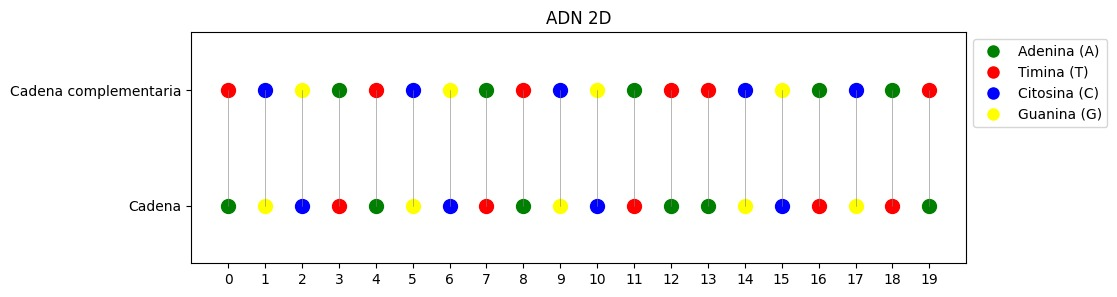
\includegraphics[scale=0.25]{adn1.jpeg} 
    \end{figure}

Aunque no utilizaremos este proceso en los siguientes pasos, mostramos cómo se realiza la transcripción de ADN a ARN y cómo se traduce el ARN a proteínas.

\begin{lstlisting}[language=Python]
arn = cadena_adn.transcribe()
print(f"Secuencia ARN: {arn}")

proteina = arn.translate()
print(f"Proteina: {proteina}")
\end{lstlisting}
Ilustrando un poco como se realiza la transcripción de ADN a ARN hicimos el siguiente gráfico
\begin{figure}[h]
\centering
        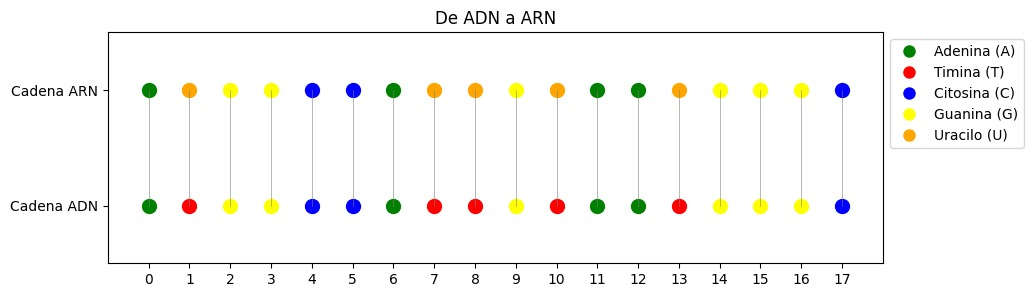
\includegraphics[scale=0.25]{arn.png} 
    \end{figure}
Utilizando todas las librerias anteriormente mencionadas realizamos la representación gráfica de la proteina a la que se puede transcribir la cadena de ARN (estas imágenes puede verlas en el archivo de código).\\


\subsection{Codificación y Decodificación con Códigos Reed-Solomon y Hamming}

En esta sección, nos adentramos en la parte central de nuestro trabajo, donde realizamos una codificación y decodificación utilizando los códigos Reed-Solomon y Hamming.

\subsubsection{Ejemplo de Corrección de Errores con Reed-Solomon}
Para ilustrar este proceso, comenzamos con un ejemplo de transcripción de ADN a ARN, donde introducimos errores en la secuencia de ARN. Luego, utilizamos los códigos Reed-Solomon para corregir estos errores, simulando el mecanismo de corrección que ocurre en la naturaleza.

\begin{lstlisting}[language=Python]
import unireedsolomon as rs
from random import choice, randint

def generar_adn(longitud):
    nucleotidos = "ATCG"
    return ''.join(choice(nucleotidos) for _ in range(longitud))

def adn_a_arn(adn):
    return adn.replace('T', 'U')


def introducir_mutaciones(sec, num_mutaciones):
    sec_lista = list(sec)
    nucleotidos = "AUCG"
    for _ in range(num_mutaciones):
        pos = randint(0, len(sec_lista) - 1)
        nucleotido_original = sec_lista[pos]
        nucleotidos_posibles = nucleotidos.replace(nucleotido_original, '')
        sec_lista[pos] = choice(nucleotidos_posibles)
    return ''.join(sec_lista)


n = 19  
k = 15  

coder = rs.RSCoder(n, k)


adn_original = generar_adn(15)
print(f"ADN original: {adn_original}")


arn_original = adn_a_arn(adn_original)
print(f"ARN original: {arn_original}")

arn_codificado = coder.encode(arn_original)
print(f"ARN codificado (hex): {arn_codificado.encode('latin1').hex()}")


arn_con_mutaciones = introducir_mutaciones(arn_codificado, 2)  # Introducir 2 mutaciones
print(f"ARN con mutaciones: {arn_con_mutaciones}")


try:
    arn_corregido, errores_corregidos = coder.decode(arn_con_mutaciones)
    print(f"ARN corregido: {arn_corregido}")
    print(f"Errores corregidos: {errores_corregidos}")
except rs.RSCodecError as e:
    print(f"Error: No se pudieron corregir todos los errores. {e}")
\end{lstlisting}

En este código se genera una cadena de ADN aleatoria de longitud especificada y esta se transcribe a ARN, reemplazando las timinas (T) por uracilos (U). Posteriormente, se introducen mutaciones en la secuencia de ARN para simular errores en la transcripción, la secuencia de ARN se codifica utilizando el código Reed-Solomon, que añaden $4$ bits de paridad para la detección y corrección de errores.\\

Este proceso es análogo a lo que ocurre en la naturaleza durante la transcripción del ADN. La enzima polimerasa revisa y corrige los errores que puedan ocurrir durante la replicación del ADN, asegurando que la información genética se transmita de manera precisa. En nuestro caso, los códigos Reed-Solomon actúan como la polimerasa, corrigiendo los errores introducidos en la secuencia de ARN.\\


En este ejemplo, el número de mutaciones introducidas es estático (2 mutaciones), ya que la idea es acercarse lo más posible a la realidad biológica. En la naturaleza, la probabilidad de que ocurran errores durante la transcripción es baja, y los mecanismos de corrección son altamente eficientes. Por esta razón, no se utilizó una matriz de transición para introducir mutaciones de manera probabilística, ya que esto reduciría la probabilidad de decodificación correcta, algo que no ocurre en el ADN.




\subsubsection{Aplicación Práctica: Codificación y Decodificación de una Palabra}

Para mostrar una aplicación análoga a lo que hace el ADN en la realidad, codificamos una palabra utilizando el código Reed-Solomon. Es importante destacar que las codificaciones no se aplican a los bits de paridad, y para utilizar completamente la librería \texttt{unireedsolomon}, realizamos una serie de conversiones. Primero, convertimos la cadena de texto a ASCII, luego a base 4, asignamos nucleótidos de ADN, introducimos ruido mediante una matriz de transición, y finalmente realizamos las conversiones inversas para decodificar la palabra. La idea principal del código es,

\begin{lstlisting}[language=Python]
palabra = input("Ingrese una palabra: ")


ascii_palabra = palabra_a_ascii(palabra)
print(f"Palabra en ASCII: {ascii_palabra}")


polinomio_palabra = polinomio(ascii_palabra)
print(f"Palabra en polinomio: {polinomio_palabra}")


def arreglar_palabra(palabra):
    palabra_coder = ''
    for i in ascii_palabra:
        palabra_coder = palabra_coder + i
    num_coder = int(palabra_coder[0:len(palabra_coder)])
    return palabra_coder

palabra_coder = arreglar_palabra(ascii_palabra)


n = len(palabra_coder) + 4
k = len(palabra_coder)


coder = rs.RSCoder(n, k)


ascii_codificado = coder.encode(palabra_coder)
print(f"Palabra codificada: {ascii_codificado}")


base4_codificado = ascii_a_base4(ascii_palabra)
print(f"Palabra codificada en base 4: {base4_codificado}")


adn_codificado = base4_a_adn(base4_codificado)
print(f"Palabra codificada en ADN: {adn_codificado}")


matriz_transicion = [
    [0.98, 0.005, 0.005, 0.01], 
    [0.005, 0.005, 0.98, 0.01], 
    [0.01, 0.005, 0.005, 0.98]   
]


adn_con_errores = introducir_errores_con_matriz(adn_codificado, matriz_transicion)
print(f"ADN con errores: {adn_con_errores}")

base4_con_errores = nucleotidos_a_base4(adn_con_errores)
print(f"Base 4 con errores: {base4_con_errores}")

ascii_con_errores = base4_a_ascii(base4_con_errores)
print(f"ASCII con errores: {ascii_con_errores}")

ascii_con_errores = ascii_con_errores + ascii_codificado[len(ascii_codificado) - 4:len(ascii_codificado)]
print(f"ASCII con errores y paridad: {ascii_con_errores}")

try:
    palabra_corregida = coder.decode(ascii_con_errores)
    print(f"Palabra corregida: {palabra_corregida}")
    palabra_final = ascii_a_palabra(palabra_corregida[0], ascii_palabra)
    print(f"Palabra final: {palabra_final}")
\end{lstlisting}

La palabra ingresada se convierte a su representación en ASCII, lo que permite trabajar con valores numéricos, los valores ASCII se convierten a base 4, lo que facilita la asignación de nucleótidos de ADN.Cada dígito en base 4 se asigna a un nucleótido (A, T, C, G) posteriormente, se utiliza una matriz de transición para introducir errores en la secuencia de ADN, simulando mutaciones.Por último se realizan las conversiones inversas para obtener la palabra original, corrigiendo los errores introducidos mediante el código Reed-Solomon.




\section{Conclusiones y Posibles direcciones}
%!TEX root = main.tex
Para finalizar, daremos unas breves reflexiones del proyecto junto a posibles direcciones futuras.
\begin{itemize}
    \item Se pudo evidenciar como de manera teórica los códigos de Reed-Solomon, al tener una fundamentación más algebraica, en su enfoque como un cádigo cáclico, resulta mucho más complicado y lleno de errores en el proceso implementación de la decodificación que el caso de los códigos de Hamming.
    \item Una de las ventajas de usar Reed-Solomon, es que al aprovechar las propiedades algebraicas de los polinomios, podemos reducir la memoria usada, ya que almacenar matrices tiene mucho mas costo. Pero este método tiene sus desventajas y es que depende del mensaje editado y el algoritmo de decodificación usado, puede que palabras que teóricamente se puedan decodificar, la implementación no pueda hacerlo.
    \item Debido a aquellas cadenas que resultaba imposible decodificar, una posible dirección futura seria realizar una implementación del código más robusta  e intentar implementar algunos de los algoritmos de decodificación para poder ver el efecto que puede tener en las cadenas donde presenta error y teóricamente no debería hacerlo.
    \item Debido a lo recientes que son los resultados en este área de investigación, las ideas tratadas en este proyecto son solo un pequeño acercamiento hacia las analogias que se pueden hacer. Por lo que para continuar por esta línea se podría primero ahondar más en los metodos usados y buscar que método resultados más eficientes, también se podría estudiar estructuras más robustas de información, debido a que en el proyecto estudiamos cadenas simples, no uniones de estas. Este enfoque podria ser aún más enriquecedor.
\end{itemize}
\bibliographystyle{unsrt}

\bibliography{references}
\nocite{*}
\end{document}


